
\documentclass[a4paper,11pt]{article}
\usepackage[a4paper, margin=8em]{geometry}

% usa i pacchetti per la scrittura in italiano
\usepackage[french,italian]{babel}
\usepackage[T1]{fontenc}
\usepackage[utf8]{inputenc}
\frenchspacing 

% usa i pacchetti per la formattazione matematica
\usepackage{amsmath, amssymb, amsthm, amsfonts}

% usa altri pacchetti
\usepackage{gensymb}
\usepackage{hyperref}
\usepackage{standalone}

\usepackage{colortbl}

\usepackage{xstring}
\usepackage{karnaugh-map}

% imposta il titolo
\title{Computer Architectures notes}
\author{Luca Seggiani}
\date{2026}

% imposta lo stile
% usa helvetica
\usepackage[scaled]{helvet}
% usa palatino
\usepackage{palatino}
% usa un font monospazio guardabile
\usepackage{lmodern}

\renewcommand{\rmdefault}{ppl}
\renewcommand{\sfdefault}{phv}
\renewcommand{\ttdefault}{lmtt}

% circuiti
\usepackage{circuitikz}
\usetikzlibrary{babel}

% testo cerchiato
\newcommand*\circled[1]{\tikz[baseline=(char.base)]{
            \node[shape=circle,draw,inner sep=2pt] (char) {#1};}}

% disponi il titolo
\makeatletter
\renewcommand{\maketitle} {
	\begin{center} 
		\begin{minipage}[t]{.8\textwidth}
			\textsf{\huge\bfseries \@title} 
		\end{minipage}%
		\begin{minipage}[t]{.2\textwidth}
			\raggedleft \vspace{-1.65em}
			\textsf{\small \@author} \vfill
			\textsf{\small \@date}
		\end{minipage}
		\par
	\end{center}

	\thispagestyle{empty}
	\pagestyle{fancy}
}
\makeatother

% disponi teoremi
\usepackage{tcolorbox}
\newtcolorbox[auto counter, number within=section]{theorem}[2][]{%
	colback=blue!10, 
	colframe=blue!40!black, 
	sharp corners=northwest,
	fonttitle=\sffamily\bfseries, 
	title=Theorem~\thetcbcounter: #2, 
	#1
}

% disponi definizioni
\newtcolorbox[auto counter, number within=section]{definition}[2][]{%
	colback=red!10,
	colframe=red!40!black,
	sharp corners=northwest,
	fonttitle=\sffamily\bfseries,
	title=Definition~\thetcbcounter: #2,
	#1
}

% disponi codice
\usepackage{listings}
\usepackage[table]{xcolor}

\definecolor{codegreen}{rgb}{0,0.6,0}
\definecolor{codegray}{rgb}{0.5,0.5,0.5}
\definecolor{codepurple}{rgb}{0.58,0,0.82}
\definecolor{backcolour}{rgb}{0.95,0.95,0.92}

\lstdefinestyle{codestyle}{
		backgroundcolor=\color{black!5}, 
		commentstyle=\color{codegreen},
		keywordstyle=\bfseries\color{magenta},
		numberstyle=\sffamily\tiny\color{black!60},
		stringstyle=\color{green!50!black},
		basicstyle=\ttfamily\footnotesize,
		breakatwhitespace=false,         
		breaklines=true,                 
		captionpos=b,                    
		keepspaces=true,                 
		numbers=left,                    
		numbersep=5pt,                  
		showspaces=false,                
		showstringspaces=false,
		showtabs=false,                  
		tabsize=2
}

\lstdefinestyle{shellstyle}{
		backgroundcolor=\color{black!5}, 
		basicstyle=\ttfamily\footnotesize\color{black}, 
		commentstyle=\color{black}, 
		keywordstyle=\color{black},
		numberstyle=\color{black!5},
		stringstyle=\color{black}, 
		showspaces=false,
		showstringspaces=false, 
		showtabs=false, 
		tabsize=2, 
		numbers=none, 
		breaklines=true
}

\lstdefinelanguage{x86}{ 
  keywords={AAA, AAD, AAM, AAS, ADC, ADCB, ADCW, ADCL, ADD, ADDB, ADDW, ADDL, AND, ANDB, ANDW, ANDL,
        ARPL, BOUND, BSF, BSFL, BSFW, BSR, BSRL, BSRW, BSWAP, BT, BTC, BTCB, BTCW, BTCL, BTR, 
        BTRB, BTRW, BTRL, BTS, BTSB, BTSW, BTSL, CALL, CBW, CDQ, CLC, CLD, CLI, CLTS, CMC, CMP,
        CMPB, CMPW, CMPL, CMPS, CMPSB, CMPSD, CMPSW, CMPXCHG, CMPXCHGB, CMPXCHGW, CMPXCHGL,
        CMPXCHG8B, CPUID, CWDE, DAA, DAS, DEC, DECB, DECW, DECL, DIV, DIVB, DIVW, DIVL, ENTER,
        HLT, IDIV, IDIVB, IDIVW, IDIVL, IMUL, IMULB, IMULW, IMULL, IN, INB, INW, INL, INC, INCB,
        INCW, INCL, INS, INSB, INSD, INSW, INT, INT3, INTO, INVD, INVLPG, IRET, IRETD, JA, JAE,
        JB, JBE, JC, JCXZ, JE, JECXZ, JG, JGE, JL, JLE, JMP, JNA, JNAE, JNB, JNBE, JNC, JNE, JNG,
        JNGE, JNL, JNLE, JNO, JNP, JNS, JNZ, JO, JP, JPE, JPO, JS, JZ, LAHF, LAR, LCALL, LDS,
        LEA, LEAVE, LES, LFS, LGDT, LGS, LIDT, LMSW, LOCK, LODSB, LODSD, LODSW, LOOP, LOOPE,
        LOOPNE, LSL, LSS, LTR, MOV, MOVB, MOVW, MOVL, MOVSB, MOVSD, MOVSW, MOVSX, MOVSXB,
        MOVSXW, MOVSXL, MOVZX, MOVZXB, MOVZXW, MOVZXL, MUL, MULB, MULW, MULL, NEG, NEGB, NEGW,
        NEGL, NOP, NOT, NOTB, NOTW, NOTL, OR, ORB, ORW, ORL, OUT, OUTB, OUTW, OUTL, OUTSB, OUTSD,
        OUTSW, POP, POPL, POPW, POPB, POPA, POPAD, POPF, POPFD, PUSH, PUSHL, PUSHW, PUSHB, PUSHA, 
        RCLL, RCR, RCRB, RCRW, RCRL, RDMSR, RDPMC, RDTSC, REP, REPE, REPNE, RET, ROL, ROLB, ROLW,
        ROLL, ROR, RORB, RORW, RORL, SAHF, SAL, SALB, SALW, SALL, SAR, SARB, SARW, SARL, SBB,
        SBBB, SBBW, SBBL, SCASB, SCASD, SCASW, SETA, SETAE, SETB, SETBE, SETC, SETE, SETG, SETGE,
        SETL, SETLE, SETNA, SETNAE, SETNB, SETNBE, SETNC, SETNE, SETNG, SETNGE, SETNL, SETNLE,
        SETNO, SETNP, SETNS, SETNZ, SETO, SETP, SETPE, SETPO, SETS, SETZ, SGDT, SHL, SHLB, SHLW,
        SHLL, SHLD, SHR, SHRB, SHRW, SHRL, SHRD, SIDT, SLDT, SMSW, STC, STD, STI, STOSB, STOSD,
        STOSW, STR, SUB, SUBB, SUBW, SUBL, TEST, TESTB, TESTW, TESTL, VERR, VERW, WAIT, WBINVD,
        XADD, XADDB, XADDW, XADDL, XCHG, XCHGB, XCHGW, XCHGL, XLAT, XLATB, XOR, XORB, XORW, XORL},
  keywordstyle=\color{blue}\bfseries,
  ndkeywordstyle=\color{darkgray}\bfseries,
  identifierstyle=\color{black},
  sensitive=false,
  comment=[l]{\#},
  morecomment=[s]{/*}{*/},
  commentstyle=\color{purple}\ttfamily,
  stringstyle=\color{red}\ttfamily,
  morestring=[b]',
  morestring=[b]"
}

\lstdefinelanguage{riscv}{
  keywords={
    LUI, AUIPC,
    JAL, JALR,
    BEQ, BNE, BLT, BGE, BLTU, BGEU,
    LB, LH, LW, LBU, LHU, LD,
    SB, SH, SW, SD,
    ADDI, SLTI, SLTIU, XORI, ORI, ANDI,
    SLLI, SRLI, SRAI,
    ADD, SUB, SLL, SLT, SLTU, XOR, SRL, SRA, OR, AND,
    ADDIW, SLLIW, SRLIW, SRAIW,
    ADDW, SUBW, SLLW, SRLW, SRAW,
    MUL, MULH, MULHSU, MULHU, DIV, DIVU, REM, REMU,
    MULW, DIVW, DIVUW, REMW, REMUW,
    LR.W, SC.W, AMOSWAP.W, AMOADD.W, AMOXOR.W,
    AMOAND.W, AMOOR.W, AMOMIN.W, AMOMAX.W,
    AMOMINU.W, AMOMAXU.W,
    LR.D, SC.D, AMOSWAP.D, AMOADD.D, AMOXOR.D,
    AMOAND.D, AMOOR.D, AMOMIN.D, AMOMAX.D,
    AMOMINU.D, AMOMAXU.D,
    FLW, FSW,
    FMADD.S, FMSUB.S, FNMSUB.S, FNMADD.S,
    FADD.S, FSUB.S, FMUL.S, FDIV.S, FSQRT.S,
    FSGNJ.S, FSGNJN.S, FSGNJX.S,
    FMIN.S, FMAX.S,
    FCVT.W.S, FCVT.WU.S, FCVT.S.W, FCVT.S.WU,
    FMV.X.W, FMV.W.X,
    FEQ.S, FLT.S, FLE.S,
    FLD, FSD,
    FMADD.D, FMSUB.D, FNMSUB.D, FNMADD.D,
    FADD.D, FSUB.D, FMUL.D, FDIV.D, FSQRT.D,
    FSGNJ.D, FSGNJN.D, FSGNJX.D,
    FMIN.D, FMAX.D,
    FCVT.W.D, FCVT.WU.D, FCVT.D.W, FCVT.D.WU,
    FCVT.S.D, FCVT.D.S,
    FMV.X.D, FMV.D.X,
    FEQ.D, FLT.D, FLE.D,
    CSRRW, CSRRS, CSRRC,
    CSRRWI, CSRRSI, CSRRCI,
    FENCE.I,
    FENCE,
    ECALL, EBREAK,
    MRET, SRET, URET,
    WFI,
    SFENCE.VMA,
    NOP, LI, LA, MV,
    NOT, NEG, NEGW,
    SEQZ, SNEZ, SLTZ, SGTZ,
    BEQZ, BNEZ, BLEZ, BGEZ, BLTZ, BGTZ,
    BGT, BLE, BGTU, BLEU,
    J, JR, RET,
    CALL, TAIL,
    RDINSTRET, RDCYCLE, RDTIME,
    CSRR, CSRW, CSRS, CSRC,
    CSRWI, CSRSI, CSRCI
  },
  keywordstyle=\color{blue}\bfseries,
  ndkeywordstyle=\color{darkgray}\bfseries,
  identifierstyle=\color{black},
  sensitive=false,
  comment=[l]{\#},
  morecomment=[s]{/*}{*/},
  commentstyle=\color{purple}\ttfamily,
  stringstyle=\color{red}\ttfamily,
  morestring=[b]',
  morestring=[b]"
}

\lstdefinelanguage{arm}{
  keywords={
    ADC, ADD, AND, BIC, CMN, CMP, EOR, MOV, MVN,
    RSB, RSC, SBC, SUB, TST, TEQ,
    MLA, MLS, MUL, SMLAL, SMULL, UMLAL, UMULL,
    QADD, QSUB, QDADD, QDSUB,
    QADD16, QADD8, QASX, QSAX,
    QSUB16, QSUB8, QSAX, QSUBADDX,
    ASR, LSL, LSR, ROR, RRX,
    B, BL, BX, BLX,
    BXJ,
    BEQ, BNE, BCS, BHS, BCC, BLO,
    BMI, BPL, BVS, BVC,
    BHI, BLS, BGE, BLT, BGT, BLE,
    BAL,
    LDR, LDRB, LDRH, LDRSB, LDRSH,
    LDRD, LDM, LDMIA, LDMIB, LDMDA, LDMDB,
    LDRT, LDRBT, LDRHT, LDRSBT, LDRSHT,
    STR, STRB, STRH, STRD,
    STM, STMIA, STMIB, STMDA, STMDB,
    STRT, STRBT, STRHT,
    PUSH, POP,
    SWP, SWPB,
    REV, REV16, REVSH,
    BFC, BFI, BFXIL, SBFX, UBFX,
    CLZ,
    LDREX, LDREXB, LDREXH, LDREXD,
    STREX, STREXB, STREXH, STREXD,
    DMB, DSB, ISB,
    MCR, MCRR, MRC, MRRC,
    MRS, MSR,
    CPS, SETEND, SVC, BKPT,
    CLREX, WFE, WFI, SEV,
    YIELD, NOP,
    VLDR, VSTR,
    VMOV, VABS, VNEG,
    VADD, VSUB, VMUL, VDIV,
    VMLA, VMLS, VNMLA, VNMLS, VNMUL,
    VMAX, VMIN,
    VSQRT,
    VCMP, VCMPE,
    VCVT,
    VCLZ, VCLS,
    VAND, VORR, VEOR, VBIC, VMVN,
    VLD1, VLD2, VLD3, VLD4,
    VST1, VST2, VST3, VST4,
    ADR, ADCS, ADDS, SUBS, MOVS, ANDS, ORRS, EORS
  },
  keywordstyle=\color{blue}\bfseries,
  ndkeywordstyle=\color{darkgray}\bfseries,
  identifierstyle=\color{black},
  sensitive=false,
  comment=[l]{@},
  morecomment=[l]{;},
  morecomment=[s]{/*}{*/},
  commentstyle=\color{purple}\ttfamily,
  stringstyle=\color{red}\ttfamily,
  morestring=[b]',
  morestring=[b]"
}

\lstset{style=codestyle, language=C}

% disponi sezioni
\usepackage{titlesec}

\titleformat{\section}
	{\sffamily\Large\bfseries} 
	{\thesection}{1em}{} 
\titleformat{\subsection}
	{\sffamily\large\bfseries}   
	{\thesubsection}{1em}{} 
\titleformat{\subsubsection}
	{\sffamily\normalsize\bfseries} 
	{\thesubsubsection}{1em}{}

% tikz
\usepackage{tikz}

% float
\usepackage{float}

% grafici
\usepackage{pgfplots}
\pgfplotsset{width=10cm,compat=1.9}

% disponi alberi
\usepackage{forest}

\forestset{
	rectstyle/.style={
		for tree={rectangle,draw,font=\large\sffamily}
	},
	roundstyle/.style={
		for tree={circle,draw,font=\large}
	}
}

% disponi algoritmi
\usepackage{algorithm}
\usepackage{algorithmic}
\makeatletter
\renewcommand{\ALG@name}{Algorithm}
\makeatother

% disponi numeri di pagina
\usepackage{fancyhdr}
\fancyhf{} 
\fancyfoot[L]{\sffamily{\thepage}}

\makeatletter
\fancyhead[L]{\raisebox{1ex}[0pt][0pt]{\sffamily{\@title \ \@date}}} 
\fancyhead[R]{\raisebox{1ex}[0pt][0pt]{\sffamily{\@author}}}
\makeatother

\begin{document}
% sezione (data)
\section{Lesson 29-09-26}

% stili pagina
\thispagestyle{empty}
\pagestyle{fancy}

% testo

\lstset{language=riscv}

\textbf{\textsf{Branches}}: we have to quickly finish up on branching instructions in the RISC-V ISA, which we left behind on the past lesson.

These are a special class of instructions: range of $\pm$ 4 KiB and a 12-bit immediate value.

\begin{center}
	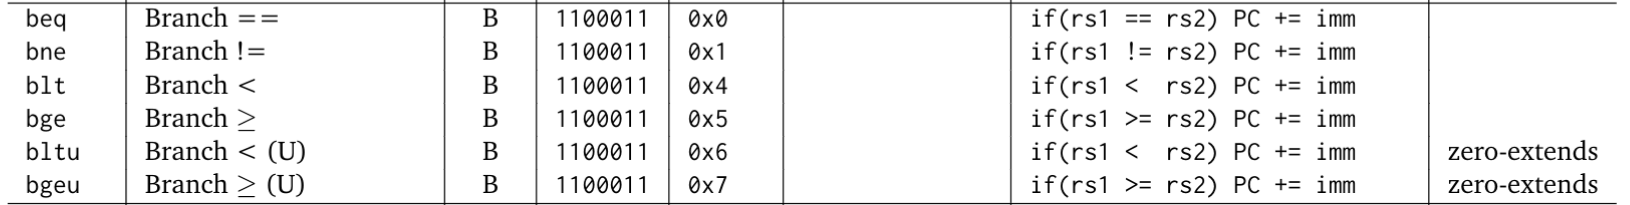
\includegraphics[scale=0.22]{../figures/riscv_branches.png}
\end{center}

The offset must be a multiple of 2, and it is added to PC on positive comparisons.
For this, branch instructions compare two registers Rs1 and Rs2

The types are a bit limited:
\begin{itemize}
	\item \lstinline|beq| and \lstinline|bne| take the branch if \lstinline|rs1| and \lstinline|rs2| are equal or unequal;
	\item \lstinline|blt| and \lstinline|bltu| take the branch if \lstinline|rs1| is less than \lstinline|rs2|;
	\item \lstinline|bge| and \lstinline|bgeu| take the branch if \lstinline|rs1| is greater than or equal to \lstinline|rs2|;
	\item \lstinline|bgt|, \lstinline|bgtu|, \lstinline|ble|, and \lstinline|bleu| can be synthesized by reversing the operands to \lstinline|blt|, \lstinline|bltu|, \lstinline|bge|, and \lstinline|bgeu|. The compiler does this automatically.
\end{itemize}

Some zero-based pseudo-instructions are availale:
\begin{itemize}
	\item \lstinline|beqz rs, label|: branches if \lstinline|rs = 0|:
\begin{lstlisting}[language=riscv, style=codestyle]	
beqz x3, label

# translates to:

beq x3, x0, label
\end{lstlisting}
	
	\item \lstinline|bnez rs, label|: branches if \lstinline|rs != 0|:
\begin{lstlisting}[language=riscv, style=codestyle]	
bnez x3, label

# translates to:

bne x3, x0, label
\end{lstlisting}

	\item \lstinline|bltz rs, label|: branches if \lstinline|rs < 0|:
\begin{lstlisting}[language=riscv, style=codestyle]	
bltz x3, label

# translates to:

blt x3, x0, label
\end{lstlisting}
	
	\item \lstinline|bgtz rs, label|: branches if \lstinline|rs1 >= 0|:
\begin{lstlisting}[language=riscv, style=codestyle]	
bgtz x3, label

# translates to:

bgt x3, x0, label
\end{lstlisting}

\end{itemize}

\subsection{Pipelining}

By studying RISC-V, we figured out that the CPU reads a sequence of fixed size instructions from memory, executing them one by one.
We know introduce an implementation technique whereby multiple instructions are overlapped in execution: we call this technique \textbf{pipelining}.
In a pipeline, different units (called pipe \textit{stages} or \textit{segments}) are (at any given time) completing different parts of different instructions in parallel.

Different stages of the pipeline perform different fixed functions on instructions.
For instance, we might have (in an undefined implementation) that the execution of each instruction may be composed of at most five clock cycles:
\begin{itemize}
	\item Instruction fetch cycle (IF)
	\item Instruction decode/register fetch cycle (ID)
	\item Execution/effective address cycle (EX)
	\item Memory access/branch completion cycle (MEM)
	\item Write-back cycle (WB).
\end{itemize}

\subsubsection{Pipeline metrics}

Let's define some \textit{metrics}.

The \textbf{throughput} of a pipelined processor is the number of instructions which exit the pipeline in the time unit.

All the pipeline stages are synchronized (they proceed to executing a new task all together): the time for executing one step is called \textbf{machine cycle}, and normally corresponds to one \textit{clock cycle}.
The length of the machine cycle is determined by the slowest stage of the pipeline.

Lastly, we define \textbf{CPI} as \textit{Clock Cycles per Instruction}.

In an ideal pipeline, all the stages are perfectly balanced (i.e., they require the same time).
The throughput of an ideal pipeline (i.e., the number of instructions completed in a given time period) is:
$$
\text{throughput}_\text{pipelined} = \text{throughput}_\text{unpipelined} * n
$$
where $n$ is the number of stages.

\subsubsection{Pipeline performance}

Pipelining increases the processor \textit{throughput} without making single instructions execution faster.
In fact, single instruction processing is made slower due to the pipeline control \textit{overhead}.
The depth of a pipeline is limited by:
\begin{itemize}
	\item The need for balanced stages;
	\item Pipelining overhead (pipeline register delay and clock skew).
\end{itemize}

\subsection{Pipeline hazards}

\textbf{Hazards} are situations that prevent an instruction from executing during its designated clock cycle.
There are three classes of hazards:
\begin{itemize}
	\item \textbf{Structural hazards}: coming from resource conflict;
	\item \textbf{Data hazards}: an instruction depends on the result of a previous instruction;
	\item \textbf{Control hazards}: depend on pipelining branches and other instructions that change the PC.
\end{itemize}

Let's see ways to deal with these hazards.

\subsubsection{Stalling}

One way of dealing with hazards is to force the pipeline to \textbf{stall}, i.e., to block instructions for one or more clock cycles.

When an instruction is stalled:
\begin{itemize}
\item The instructions following the stalled instruction are also stalled;
\item The instructions preceding the stalled instruction continue.
\end{itemize}
This can be easily achieved by modifying the buffer registers, making them able to \textit{conserve} the previous value (this will be the sstage which caused the hazard), and introducing an empty instruction to propagate onwards.

A stall causes the introduction of a \textit{"bubble"} in the pipeline, which has to propagate through the whole pipeline.

This is the simplest way to solve pipeline hazards, as waiting it out (eventually) solves all problems.

\subsubsection{Structural hazards}

\textbf{Structural hazards} may happen when some pipeline unit is not able to execute all the operations scheduled for a given cycle.
This is usually tied to limited resources in the processor.

Some common examples are:
\begin{itemize}
	\item A given unit is not able to complete its task in one clock cycle;
	\item The pipeline owns only one register-file write port, but there are cycles in which two register writes are required;
	\item The pipeline refers to a single-port memory, and there are cycles in which different instructions would like to access to the memory together.
\end{itemize}

\par\smallskip
\textbf{\textsf{Solution}}

Removing structural hazards requires adding new hardware or improving the existing one.
The designer has to trade-off between performance (add more resources or keep stalling) and cost (add more resources or keep the ones you have), basing on the frequency of occurrence of structural hazards.

This calls for optimization.
Let's consider \textit{load structural hazards}: these happen when two instructions contemporarily try to make a memory access to a single-port memory.
The clear solution is to split instruction and data memory.

Assume that:
\begin{itemize}
	\item $40 \%$ of instructions access the memory;
	\item The machine with the structural hazard has a clock $1.05$ times faster than the one without.
\end{itemize}

We want to measure the performance gain.

\begin{itemize}
	\item 
For the machine without structural hazard:
$$
\text{Average Instruction Time}' = CPI \times T_C 
$$
where $T_C$ is the clock period.

	\item
For the machine with structural hazard:
$$
\text{Average Instruction Time}'' = CPI_\text{ideal} \times T''_c + \text{Inst. freq} \times \text{Stall penalty}
$$
computed using $T''_C = T_C \times 1.05$.
\end{itemize}

\subsubsection{Data hazards}

Overlapping the execution of instructions, as it is done by pipelining, changes the order of read/write accesses to operands:
This can result in:
\begin{itemize}
	\item Wrong results;
	\item Undeterministic behavior.
\end{itemize}

We call these \textbf{data hazards}.

Let's consider the code fragment:
\begin{lstlisting}[language=riscv, style=codestyle]	
add r1,  r2, r3  # r1 write 

sub r4,  r1, r5  # r1 read from here onwards !
and r6,  r1, r7
or  r8,  r1, r9
xor r10, r1, r11
\end{lstlisting}

The problem is that the ADD instruction writes the result in R1 in the WB stage.
\begin{itemize}
	\item The SUB instruction reads R1 in its ID stage, two clock cycles before the one in which R1 is made available (one to feed R1 to WB and one to let WB finish): this produces a wrong result;
	\item The AND instruction reads R1 in its ID stage, one clock cycle before the one in which R1 is made available: this produces a wrong result;
	\item The OR instruction reads R1 in its ID stage, in the same clock cycle in which R1 is made available: this produces a correct result, provided that the write accesses to the register file are made before the read accesses. From now ownrads, until we write R1 again,the results are correct (XOR is correct).
\end{itemize}

Another scenario in which we encounter data hazards is because of \textit{interrupt effects}.
If an interrupt occurs during the execution of a critical piece of code (from the point of view of data hazards), correctness may actually be restored (as instructions leave the pipeline as the interrupt is handled).
This may cause an undeterministic behavior.

\par\smallskip
\textbf{\textsf{Solution}}

The typical solution to data hazards is that of \textbf{forwarding}.
A special hardware in the datapath detects when a previous ALU operation should write the register corresponding to the source of the current ALU operation.
In this case, the hardware selects the ALU result as the ALU input rather than the value from the register file.

For this to be implemented, the hardware must be able:
\begin{itemize}
	\item To forward a data from any of the previously started instructions (provided that they didn’t already write the data in its final location);
	\item Not to forward anything, if the following instruction is stalled, or an interrupt occurred.
\end{itemize}

\par\smallskip

Forwarding can also be \textbf{generalized}: in order to always avoid stalling, it should be made possible between any pipeline register to any input of any functional unit.

\subsection{Datapath model}

Let's look at a simplified \textbf{datapath} schematic to explain pipelines with more detail.

\begin{center}
	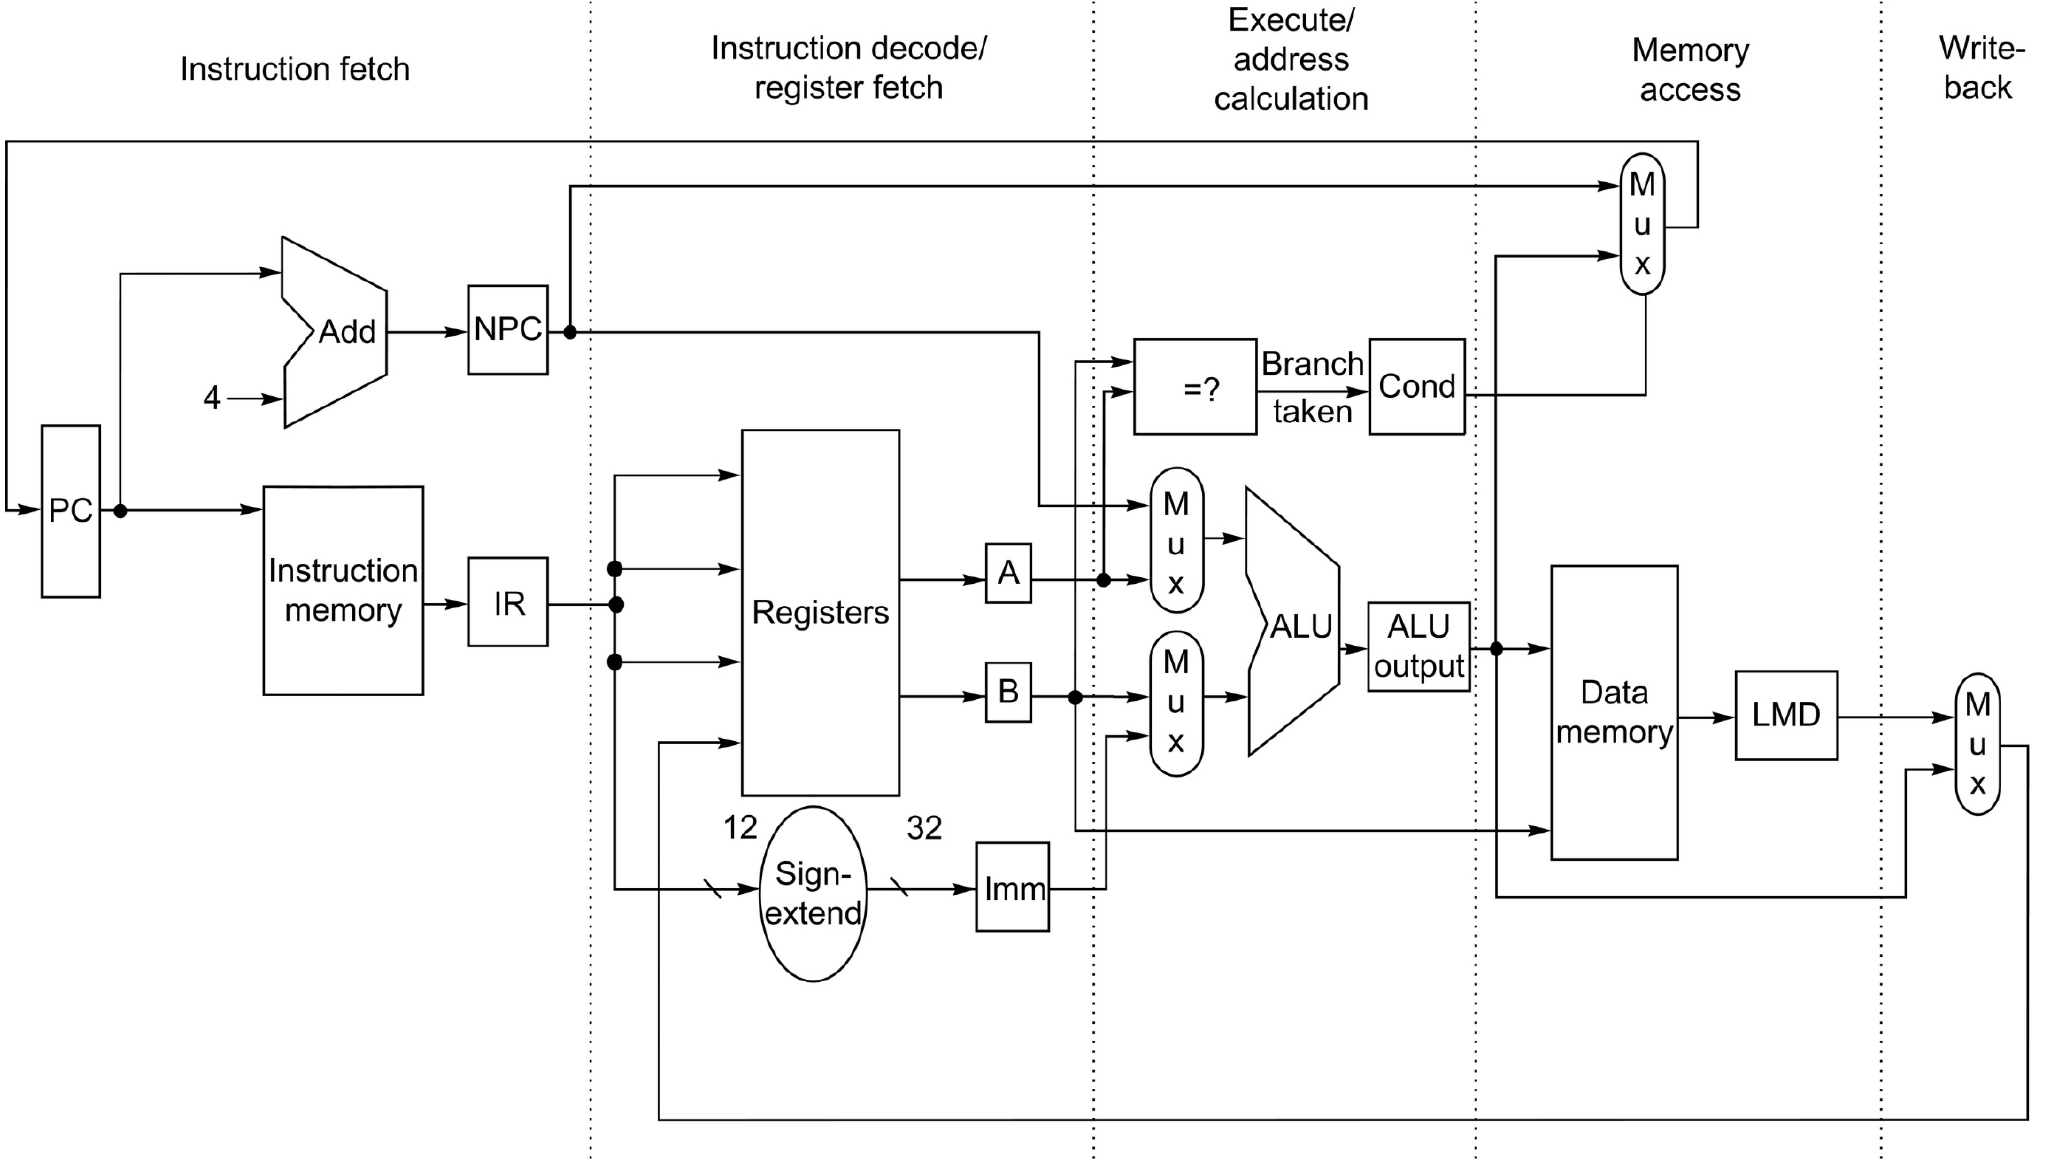
\includegraphics[scale=0.28]{../figures/datapath.png}
\end{center}

\subsubsection{Instruction fetch}

The \textbf{instruction fetch} stage has the job of fetching the next instruction from program memory and feeding it to the next stage.

As we can see, we use the \textbf{PC} (\textit{Program Counter}) to index instruction memory and put the instruction data into the \textbf{IR} (\textit{Instruction Register}).
Then we increment the program counter by 4 bytes (the size of a RISC-V instruction) and put that into an \textbf{NPC} (\textit{New Program Counter}) register.

\subsubsection{Instruction decode}

We then have to \textbf{decode} the instruction.

A number of fields are extracted from the instruction encoding (we saw that RISC-V is highly regular).
This allows for \textit{fixed-field decoding}: decoding can be performed while registers are read.

\begin{itemize}
	\item Parts of the instruction that index \textit{registers} index the \textbf{register file}. In this example we index two registers, $A$ and $B$;
	\item The immediate operand is also extracted from the instruction encoding, sign extended and sent to the next stage.
\end{itemize}

We can say that this stage performs both \textbf{decoding} and \textbf{register fetching}.

\subsubsection{Instruction execution}

At this point we can \textbf{execute} the instructions.

This is performed through the \textbf{ALU} (\textit{Arithmetic Logic Unit}), which is basically a big multiplexer of different computation circuits.

We also have to distinguish between input registers and immediates (through multiplexers).
Let's look at a couple of instruction types as an example:
\begin{itemize}
	\item \textit{Memory reference}: $\text{ALU output} \leftarrow A + Imm$. Note that we store the target \textit{address} of the memory access! For loads we will use this directly, for stores we will use $B$ and write the ALU output;
	\item \textit{Register-Register ALU instruction}: $\text{ALU output} \leftarrow A \, \text{funct} \, B$
	\item \textit{Register-Register ALU instruction}: $\text{ALU output} \leftarrow A \, \text{funct} \, \text{Immediate}$
	\item \textit{Branch}: $\text{ALU output} \leftarrow NPC + \text{Immediate} << 2$, $Cond \leftarrow (A == B)$
\end{itemize}

Another thing to note is if the instruction is a branch one: if it is, we have to evaluate a condition and use it to multiplex between NPC and a calculated value (here the value of register $A$).

We can say that this stage performs both \textbf{execution} and \textbf{address calculation}.

\subsubsection{Memory access}

An extra stage is given by the \textbf{memory access} stage.

\begin{itemize}
	\item If a (\textbf{load}) instruction requires it, we use the ALU output to address memory and load the needed contents in the \textbf{LMD} (\textit{Loaded Memory Data}) register;
	\item If a (\textbf{store}) instruction requires it, we use the $B$ register to address memory, and write the ALU output to it.
\end{itemize}

This is also the stage where we perform the \textit{branch completion cycle}, that is decide if we should update the NPC or keep it at $\text{PC} + 4$.

More clearly:
\begin{itemize}
	\item \textit{Memory reference}: $LMD \leftarrow \text{Mem}[\text{ALUOutput}]$ (loads) or $\text{Mem}[\text{ALUOutput}] \leftarrow B$ (stores);
	\item \textit{Branch}:
$$
cond \ ?\  PC \leftarrow \text{ALU output}, \ \text{otherwise} \ PC \leftarrow NPC
$$
\end{itemize}

\subsubsection{Write-back cycle}

The last step to perform is the \textbf{write-back}.

Based on the instruction type, we update the register file with the obtained result:
\begin{itemize}
	\item \textit{Register-to-register} or \textit{register-to-memory} instructions feed the ALU output to the register file;
	\item \textit{Load} instructions feed the LMD to the register file.
\end{itemize}

More clearly:
\begin{itemize}
	\item \textit{Register-Register ALU instruction}: $\text{Regs}[IR11.7] \leftarrow \text{ALU output}$;
	\item \textit{Register-Immediate ALU instruction}: $\text{Regs}[IR11.7] \leftarrow \text{ALU output}$;
	\item \textit{Load instruction}: $\text{Regs}[IR11.7] \leftarrow LMD$;
\end{itemize}

\par\smallskip

In this discussion we skipped a lot of details about the implementation, for instance how the multiplexers are driven, etc...
We assume these details to be (more or less) easy to synthesize as combinatorial or sequential networks once an actual architecture is defined.

\par\smallskip

In the described architecture, all instructions require 5 clock cycles, except branch instructions, which require 4 clock cycles.
Optimizations could be done for reducing the average CPI: as an example, the ALU instructions could be completed during the memory access cycle.
Also, hardware resources could be optimized by avoiding duplications (e.g., for ALUs, and memory).
An alternative single-clock architecture (i.e., executing an instruction per clock cycle) can also be considered, but in that case a simple control unit is required to produce the signals required by the datapath.

\subsubsection{Pipelined version}

A different solution can be using a \textbf{pipelined} version, where a new instruction is started at each clock cycle.
Different resources work on different instructions at the same time, and at every clock cycle, each resource can be used for one purpose, only.
This means that:
\begin{itemize}
	\item Separate instruction and data memories (i.e., caches) must be used;
	\item The register file is used in two stages: for reading (second half of the cycle) in ID and for writing (first half of the cycle) in WB. It must be designed to satisfy these requests during the same clock cycle.
	\item The PC must be changed in the IF stage, and branch handling must be considered;
	\item \textit{Pipeline registers} must be added between stages to act as buffers.
\end{itemize}

\begin{center}
	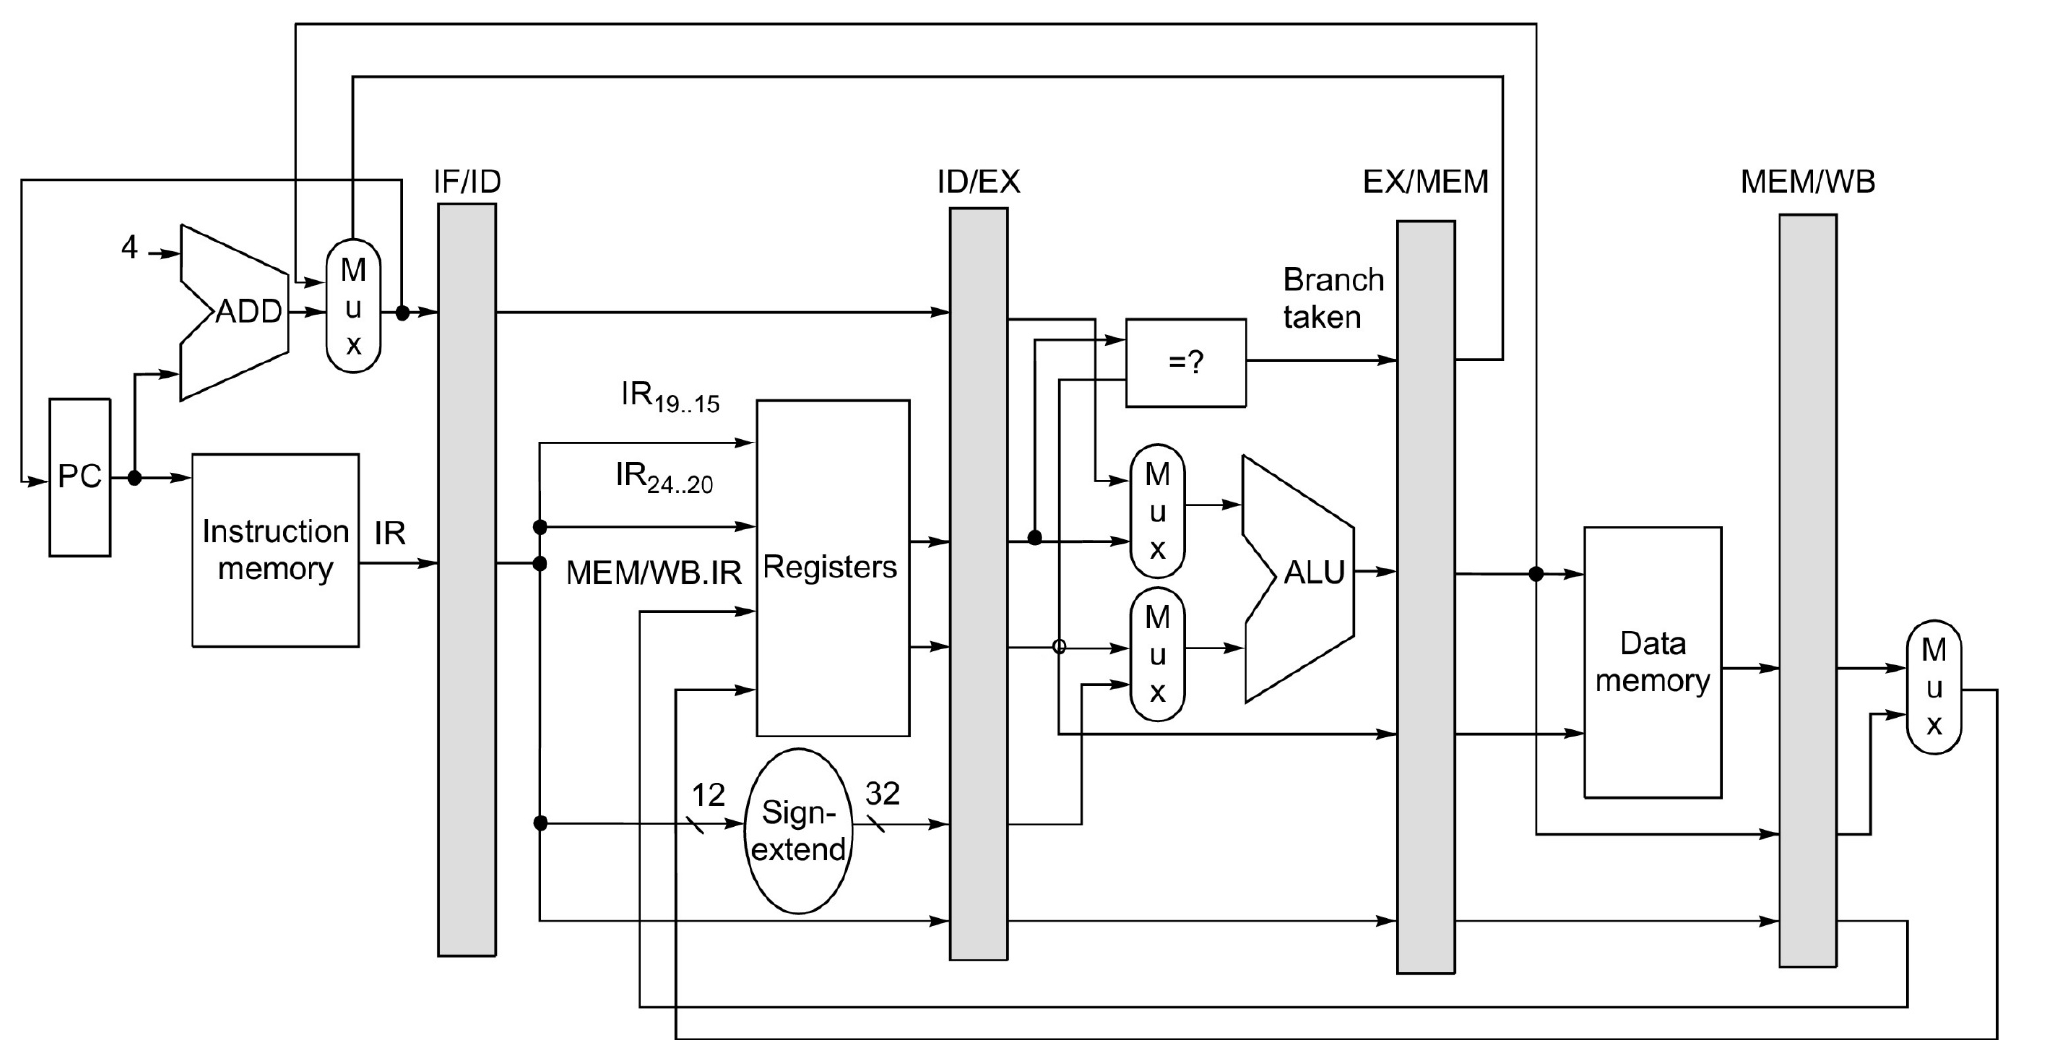
\includegraphics[scale=0.28]{../figures/datapath_pipeline.png}
\end{center}

\subsubsection{Structural hazard control}

We don't go in depth on \textbf{structural hazard} control as we saw that it depends on the resources available to the processor.
The solution remains \textit{stalling}.

\subsubsection{Data hazard load control}

Let's first go over the \textbf{causes} of data hazards.

\par\smallskip
\textbf{\textsf{Causes}}

A hazard is created whenever there is dependence between instructions, and they are close enough that the overlap caused by pipelining would change the order of access to an operand.
In general, this can happen for:
\begin{itemize}
	\item \textbf{Register operands};
	\item \textbf{Memory operands}: this is possible if:
	\begin{itemize}
		\item Accesses to memory by load and store are not made in the same stage;
		\item Execution can proceed while an instruction waits for a cache miss to be solved.
	\end{itemize}
\end{itemize}

A problem is that not all data hazards can be solved through data forwarding.
Focusing on \textbf{loads}, let's consider the code fragment:
\begin{lstlisting}[language=riscv, style=codestyle]	
ld  r1, 0(r2)  # r1 loaded 

sub r4, r1, r5 # r1 used
and r6, r1, r7
or  r8, r1, r9
\end{lstlisting}

Here, when \lstinline|sub| enters the execution stage, the data memory access is just being initiated on instruction \lstinline|ld|.
The forwarding path here goes back in time, therefore it is impossible to implement.
This means it's impossible to forward: our only solution is a stall.

\par\smallskip
\textbf{\textsf{Load control}}

Implementing the \textbf{control} for these bubbles requires that at each clock cycle:
\begin{itemize}
	\item All tests for detecting a possible data hazard concerning an instruction are performed when this is in the ID stage
	\item If a data hazard is detected, two actions can be alternatively taken:
	\begin{itemize}
		\item The appropriate forwarding is activated;
		\item The instruction is stalled before entering the stage where operands are not available (i.e., before being issued).
	\end{itemize}
\end{itemize}

\par\smallskip

The control circuitry used to handle loads is called \textbf{LID} (\textit{Load Interlock Detection}).

Let's look at a table of possible hazard conditions:
\begin{table}[H]
\centering
\begin{tabular}{lll}
\textbf{Situation} & \textbf{\begin{tabular}[c]{@{}l@{}}Example fragment\end{tabular}} & \textbf{Action} \\ \hline
No dependence & \begin{tabular}[c]{@{}l@{}}\texttt{LD   R1,45(R2)}\\\texttt{DADD R5,R6,R7}\\\texttt{DSUB R8,R6,R7}\\\texttt{OR   R9,R6,R7}\end{tabular} & \begin{tabular}[c]{@{}l@{}}No hazard possible because no dependence\\ exists on R1 in the immediately following three\\ instructions.\end{tabular} \\ \hline
\begin{tabular}[c]{@{}l@{}}Dependence\\ requiring stall\end{tabular} & \begin{tabular}[c]{@{}l@{}}\texttt{LD   \textbf{R1},45(R2)}\\\texttt{DADD R5,\textbf{R1},R7}\\\texttt{DSUB R8,R6,R7}\\\texttt{OR   R9,R6,R7}\end{tabular} & \begin{tabular}[c]{@{}l@{}}Comparators detect the use of R1 in the DADD\\ and stall the DADD (and DSUB and OR) before the\\ DADD begins EX.\end{tabular} \\ \hline
\begin{tabular}[c]{@{}l@{}}Dependence\\ overcome by\\ forwarding\end{tabular} & \begin{tabular}[c]{@{}l@{}}\texttt{LD   \textbf{R1},45(R2)}\\\texttt{DADD R5,R6,R7}\\\texttt{DSUB R8,\textbf{R1},R7}\\\texttt{OR   R9,R6,R7}\end{tabular} & \begin{tabular}[c]{@{}l@{}}Comparators detect use of R1 in DSUB and\\ forward result of load to ALU in time for DSUB\\ to begin EX.\end{tabular} \\ \hline
\begin{tabular}[c]{@{}l@{}}Dependence with\\ accesses in order\end{tabular} & \begin{tabular}[c]{@{}l@{}}\texttt{LD   \textbf{R1},45(R2)}\\\texttt{DADD R5,R6,R7}\\\texttt{DSUB R8,R6,R7}\\\texttt{OR   R9,\textbf{R1},R7}\end{tabular} & \begin{tabular}[c]{@{}l@{}}No action required because the read of R1 by OR\\ occurs in the second half of the ID phase, while\\ the write of the loaded data occurred in the first\\ half.\end{tabular} \\
\end{tabular}
\end{table}

We deduce that the following checks have to be performed when a load instruction is in the EX stage and another instruction exploiting the loaded value is in the ID stage.

\begin{table}[h!]
	\center \rowcolors{2}{white}{black!10}
	\begin{tabular} { c | c | c }
		\bfseries ID Opcode & \bfseries IF Opcode & \bfseries Match \\
		\hline
		Load & Register-Register ALU & ID/EX.IR[rd] == IF/ID.IR[rs1] \\
		Load & Register-Register ALU & ID/ EX.IR[rd] == IF/ID.IR[rs2] \\
		Load & Load, store, ALU immediate, branch & ID/EX.IR[rd] == IF/ID.IR[rs1] \\
	\end{tabular}
\end{table}

If operands match, a data hazard is detected and as a result, the control unit must insert a pipeline stall and prevent the instructions in IF and ID stages from advancing.

\par\smallskip

At this point, given an instruction currently in the ID stage, introducing a stall in the EX stage can be done by:
\begin{itemize}
	\item Forcing a nop instruction in the ID/EX pipeline register (in RISC-V the nop corresponds to an \lstinline|addi x0, x0, 0|);
	\item Forcing the IF/ID pipeline register to maintain the current value (\textit{conserve});
	\item Freezing the PC (maintain unaltered IF status).
\end{itemize}

\subsubsection{Data hazard forwarding control}

Note that the above table only pertains to \textit{load} operations, that is situations when we are \textit{loading} some data from memory and an instruction wants to access that data while the load is still happening in the pipeline.

We said that there can also be \textit{register} hazards, so now let's shift our attention to a method of solving them, that is \textbf{forwarding}.
This being said, in a special case (row 4 of the table at 4.3.8) load instructions can also benefit from forwarding from MEM to EX.

SO to summarize, forwarding can be implemented:
\begin{itemize}
	\item From the ALU or data memory output;
	\item To ALU inputs, data memory inputs, or the zero detection unit (branch instructions).
\end{itemize}

The forwarding logic must compare:
\begin{itemize}
	\item The destination fields of the IR contained in the EX/MEM and MEM/WB registers;
	\item The source fields of the IR contained in the IF/ID, ID/EX and EX/MEM registers.
\end{itemize}

We see one final table regarding the forwarding conditions and the \textit{comparisons} (checks): 
\begin{table}[H]
\center \rowcolors{2}{white}{black!10}
\small
\begin{tabular}{p{2cm} | p{2cm} | p{2cm} | p{2cm} | p{2cm} | p{2cm}}
\textbf{Source} & \textbf{Opcode} &
\textbf{Dest.} & \textbf{Opcode} &
\textbf{Forward} & \textbf{Comparison} \\ \hline

EX/MEM & Reg--reg ALU, ALU imm. &
ID/EX & Reg--reg ALU, ALU imm., load, store, branch &
Top ALU &
\texttt{EX/MEM.rd == ID/EX.rs1} \\

EX/MEM & Reg--reg ALU, ALU imm. &
ID/EX & Reg--reg ALU &
Bottom ALU &
\texttt{EX/MEM.rd == ID/EX.rs2} \\

MEM/WB & Reg--reg ALU, ALU imm., load &
ID/EX & Reg--reg ALU, ALU imm., load, store, branch &
Top ALU &
\texttt{MEM/WB.rd == ID/EX.rs1} \\

MEM/WB & Reg--reg ALU, ALU imm., load &
ID/EX & Reg--reg ALU &
Bottom ALU &
\texttt{MEM/WB.rd == ID/EX.rs2}

\end{tabular}
\end{table}

\subsubsection{Summary of RISC-V dependency handling}

To summarize, we note that the following situations might happen in the pipeline, and the tools we have available to solve them:

\begin{table}[H]
	\center \rowcolors{2}{white}{black!10}
	\begin{tabular}{ p{7cm} | p{7cm} }
		\bfseries Situation & \bfseries Solution \\
		\hline
		No dependence & Do nothing \\
		Structural hazard & Stall \\
		Any source IF/ID register in load target ID/EX stage & Stall (table 1) \\
		Any reg-reg ID/EX register in any target EX/MEM stage & Forward (table 2) \\
		Any reg-reg or load ID/EX register in any target MEM/WB stage & Forward (table 2) \\
	\end{tabular}
\end{table}

Exact register comparisons are found in the tables above.
Table 1 refers to the \textit{load control} table, wherease table 2 refers to the \textit{forwarding control} table.
It's clear that we are forced to stall only on structural and load dependencies (so when the data physically isnt in the CPU at the needed time).

\par\smallskip

For clarity (and also for fun) we test these out on a microarchitectural simulator.
The simulator chosen is \textbf{Gem5} (\url{https://www.gem5.org/}) as it's used by the course.

A code example is provided, and underneath the disassembly without pseudo-instructions and pipeline state.
It should be clear that the hazards in table 1 (section 4.3.8) are solved via stalling, whereas the hazards in table 2 (section 4.3.9) are solved, if the processor supports it, via forwarding. 

\begin{enumerate}

\item \textbf{Table 1} (4.3.8), \textbf{type 1}: ALU source register 1 target of load.

\begin{lstlisting}[language=riscv, style=codestyle]	
.section .data
    val: .word 42

# The text section contains the instructions that the CPU runs.
.section .text
# Make _start visible as the point where the program begins.
.globl _start
_start:

# setup load
    la t0, val

# perform test a
    lw t1, 0(t0)
    add t5, t1, t2

# The End block stops the program and returns control to the simulator.
End:
    li a0, 0
    li a7, 93
    ecall
\end{lstlisting}

\begin{center}
	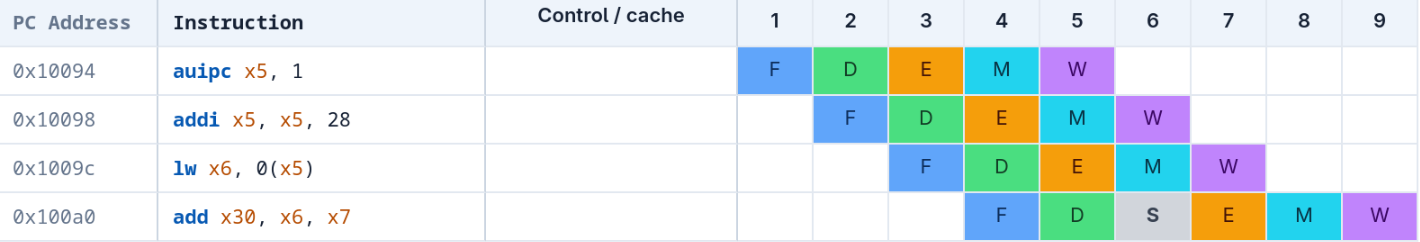
\includegraphics[scale=0.36]{../figures/riscv_deps/4_3_8_a.png}
\end{center}

\item \textbf{Table 1} (4.3.8), \textbf{type 2}: ALU source register 2 target of load.

\begin{lstlisting}[language=riscv, style=codestyle]	
.section .data
    val: .word 42

# The text section contains the instructions that the CPU runs.
.section .text
# Make _start visible as the point where the program begins.
.globl _start
_start:

# setup load
    la t0, val

# perform test a
    lw t1, 0(t0)
    add t5, t2, t1

# The End block stops the program and returns control to the simulator.
End:
    li a0, 0
    li a7, 93
    ecall
\end{lstlisting}

\begin{center}
	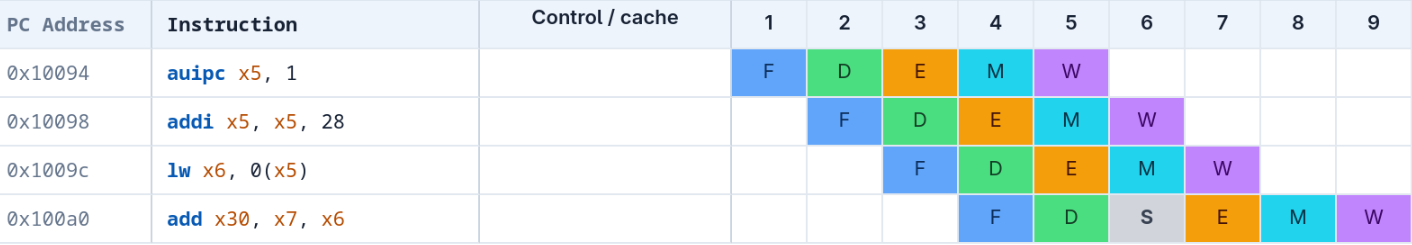
\includegraphics[scale=0.36]{../figures/riscv_deps/4_3_8_b.png}
\end{center}

\item \textbf{Table 1} (4.3.8), \textbf{type 3}: load source target of (other) load.

\begin{lstlisting}[language=riscv, style=codestyle]	
.section .data
val:  .byte 42
addr: .word val

# The text section contains the instructions that the CPU runs.
.section .text
# Make _start visible as the point where the program begins.
.globl _start
_start:

# setup load
    la t1, addr

# perform test c
    lw t2, 0(t1)
    lb t3, 0(t2)

# The End block stops the program and returns control to the simulator.
End:
    li a0, 0
    li a7, 93
    ecall
\end{lstlisting}

\begin{center}
	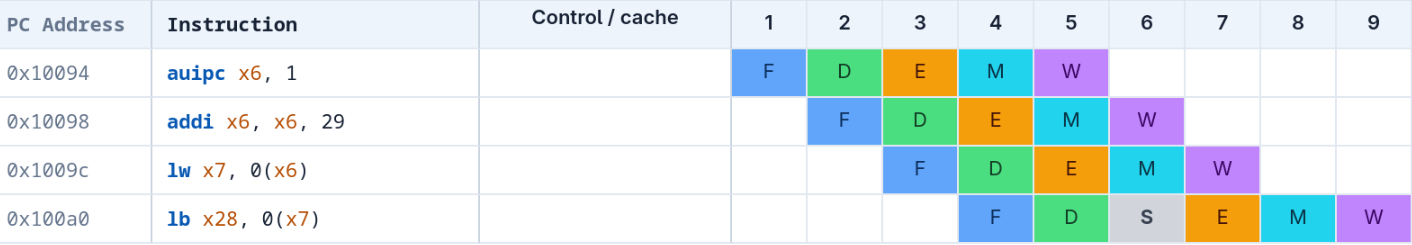
\includegraphics[scale=0.36]{../figures/riscv_deps/4_3_8_c.png}
\end{center}

\item \textbf{Table 2} (4.3.9), \textbf{type 1}: ALU source register 1 target of ALU.

\begin{lstlisting}[language=riscv, style=codestyle]	
# The text section contains the instructions that the CPU runs.
.section .text
# Make _start visible as the point where the program begins.
.globl _start
_start:

# setup registers
    li t2, 2
    li t3, 2
    li t5, 2
    nop

# perform test a
    add t1, t2, t3
    sub t4, t1, t5

# The End block stops the program and returns control to the simulator.
End:
    li a0, 0
    li a7, 93
    ecall
\end{lstlisting}

\begin{center}
	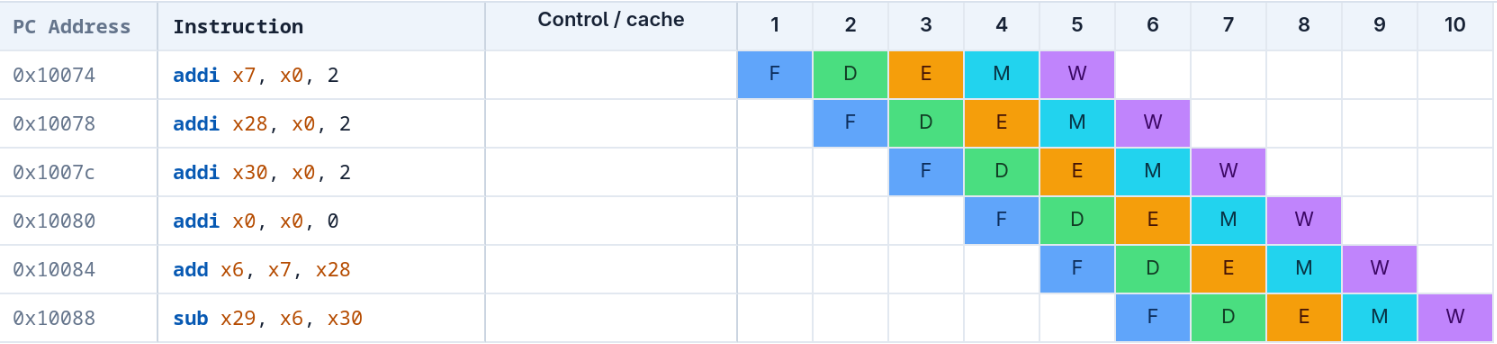
\includegraphics[scale=0.36]{../figures/riscv_deps/4_3_9_a.png}
\end{center}

\item \textbf{Table 2} (4.3.9), \textbf{type 1}: ALU source register 2 target of ALU.

\begin{lstlisting}[language=riscv, style=codestyle]	
# The text section contains the instructions that the CPU runs.
.section .text
# Make _start visible as the point where the program begins.
.globl _start
_start:

# setup registers
    li t2, 2
    li t3, 2
    li t5, 2
    nop

# perform test a
    add t1, t2, t3
    sub t4, t5, t1

# The End block stops the program and returns control to the simulator.
End:
    li a0, 0
    li a7, 93
    ecall
\end{lstlisting}

\begin{center}
	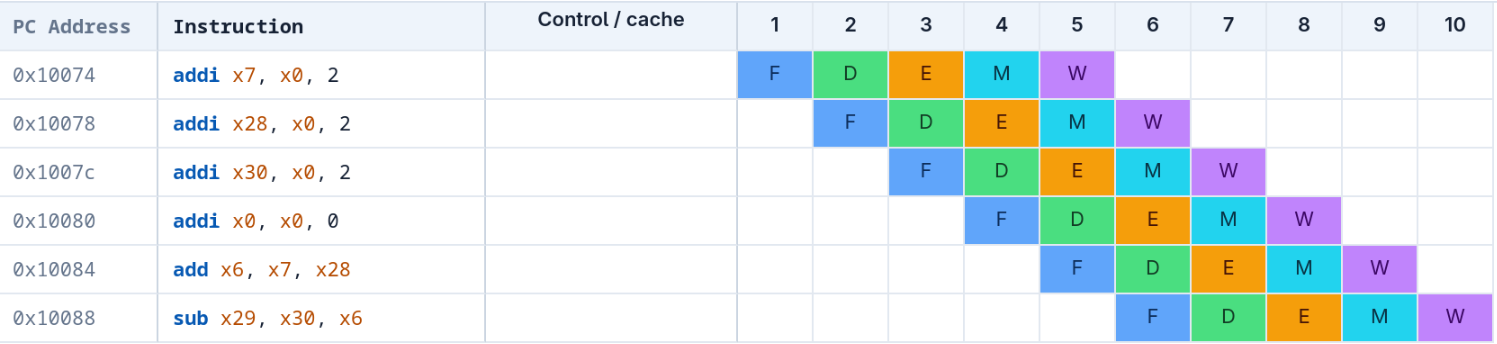
\includegraphics[scale=0.36]{../figures/riscv_deps/4_3_9_b.png}
\end{center}

\item \textbf{Table 2} (4.3.9), \textbf{type 1}: ALU source register 1 target of load (delayed).

\begin{lstlisting}[language=riscv, style=codestyle]	
.section .data
val: .byte 3

# The text section contains the instructions that the CPU runs.
.section .text
# Make _start visible as the point where the program begins.
.globl _start
_start:

# setup load
    la t0, val
    li t6, 2
    nop

# perform test c
    lb t1, 0(t0)
    nop # or anything else that doesn't touch t1
    add t5, t1, t6

# The End block stops the program and returns control to the simulator.
End:
    li a0, 0
    li a7, 93
    ecall
\end{lstlisting}

\begin{center}
	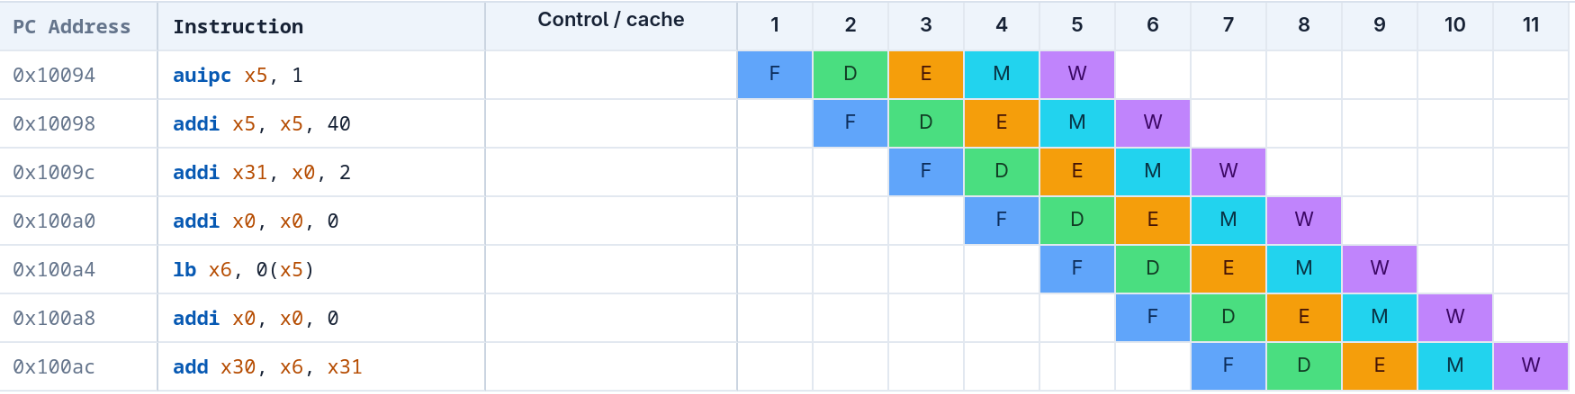
\includegraphics[scale=0.36]{../figures/riscv_deps/4_3_9_c.png}
\end{center}

\item \textbf{Table 2} (4.3.9), \textbf{type 1}: ALU source register 2 target of load (delayed).

\begin{lstlisting}[language=riscv, style=codestyle]	
.section .data
val: .byte 3

# The text section contains the instructions that the CPU runs.
.section .text
# Make _start visible as the point where the program begins.
.globl _start
_start:

# setup load
    la t0, val
    li t6, 2
    nop

# perform test c
    lb t1, 0(t0)
    nop # or anything else that doesn't touch t1
    add t5, t6, t1

# The End block stops the program and returns control to the simulator.
End:
    li a0, 0
    li a7, 93
    ecall
\end{lstlisting}

\begin{center}
	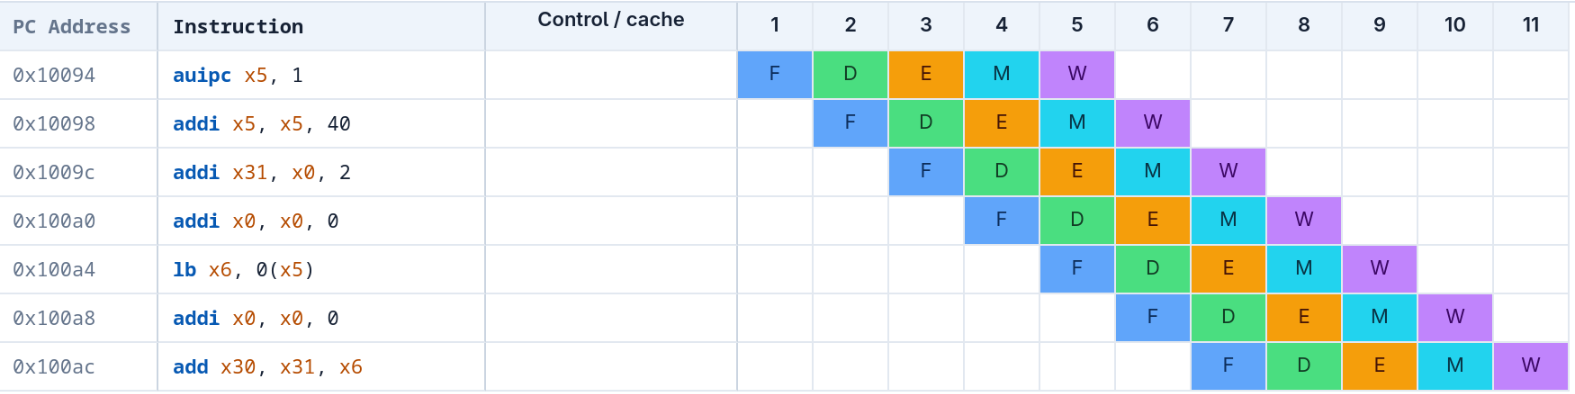
\includegraphics[scale=0.36]{../figures/riscv_deps/4_3_9_d.png}
\end{center}

\end{enumerate}

\end{document}
